\section{Results}

\subsection{Participants}

A total of 28 participants (13 female), mean age 30.7 years (SD = 10.6), volunteered to participate in the experiment. The participants, for the greater part customers of the local climbing gym, were mainly lead climbers (23) but also top-rope climbers (4) and one boulderer. The average \glsdisplay{UIAA}{UIAA} climbing degree (level of difficulty) of the lead climbers was 6+ ($\pm$1 degree), and of the top-rope climbers 5+/6- ($\pm$1 degree). About three quarters of the participants climb at least once a week. 26 out of 28 participants had never (13) used a VR system prior to the experiment or only once (13); the remaining two participants had used various systems frequently before. All participants provided written informed consent. Due to technical issues, some recordings were missing or incomplete resulting in a reduced sample size for some statistics. All relevant measurements are listed in Table \vref{tab:measurement-results}.

We used the German short version of the \glsfirst{STAI} as a standard check to measure trait anxiety \autocites{Pijpers2006}{Grimm2009}[based on][]{Spielberger1970}. This inventory consists of ten items and results in a score between 20 (low) to 80 (high), which indicates the participants' tendency of responding to situations perceived as thrilling with an elevation of \textit{state} anxiety. The overall mean \textit{trait} anxiety was 34.9 (SD = 14.9). Neither female (36.1, SD = 15.7) nor male participants (33.8, SD = 14.6) showed significant differences from scores originally surveyed by \textcite{Spielberger1983}, for adults between 19 and 39 years, of 36.15 (SD = 9.53) and 35.55 (SD = 9.76), respectively. Hence, these results indicate that the participants had no extraordinary tendency to respond to situations perceived as threatening with an elevation in state anxiety \autocites{Pijpers2006}[based on][]{smith1998measurement}.

To identify participants who fulfill the psychiatric criteria of acrophobia, we asked them to answer the \gls{vHI} questionnaire by \textcite{Huppert2017}. This questionnaire has an opening question followed by eight items and results in a severity score (vHISS) between 0 (low) and 13 (high). With two additional questions, a diagnosis of acrophobia can be established. The \gls{vHI} questionnaire was only shown to the 16 participants who affirmed the opening question; non of them got diagnosed with acrophobia and the average severity score was 1.4 (SD = 0.16).

In the following subsections, we report the results gathered from the measurements and self-reports for the three conditions of our experiment: \textit{\ref{cd:A},} climbing in reality, \textit{\ref{cd:B},} climb in \gls{VR} with props, and \textit{\ref{cd:C},} climb in \gls{VR} with controllers. First, the level of physical exertion is examined to ensure we only compare homogeneous conditions later on. Then we continue with the outcomes for stress and anxiety, and, finally, presence, which we conclude our report with. All measurement results are listed in Table \vref{tab:measurement-results}.

\begin{figure}[htb]
	\centering
	\begin{subfigure}[t]{0.49\columnwidth}
		\centering
		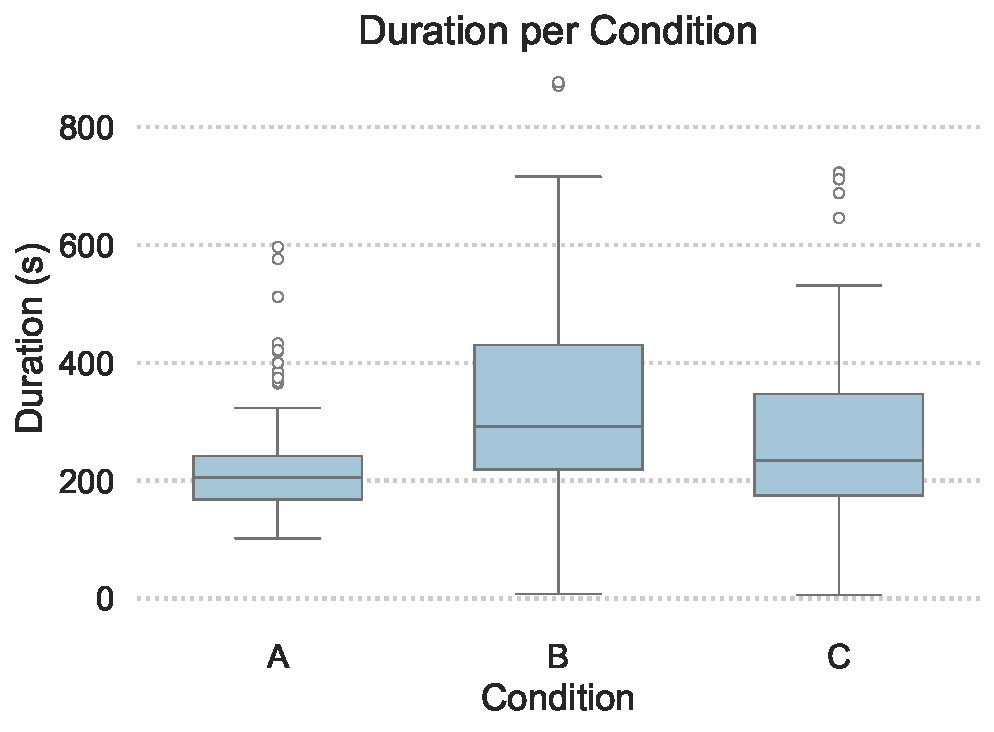
\includegraphics[width=\textwidth]{include/images/duration_per_condition.pdf}
		\caption{Duration per condition}
		\label{fig:duration-condition}
	\end{subfigure}
	\hspace*{\fill}
	\begin{subfigure}[t]{0.49\columnwidth}
		\centering
		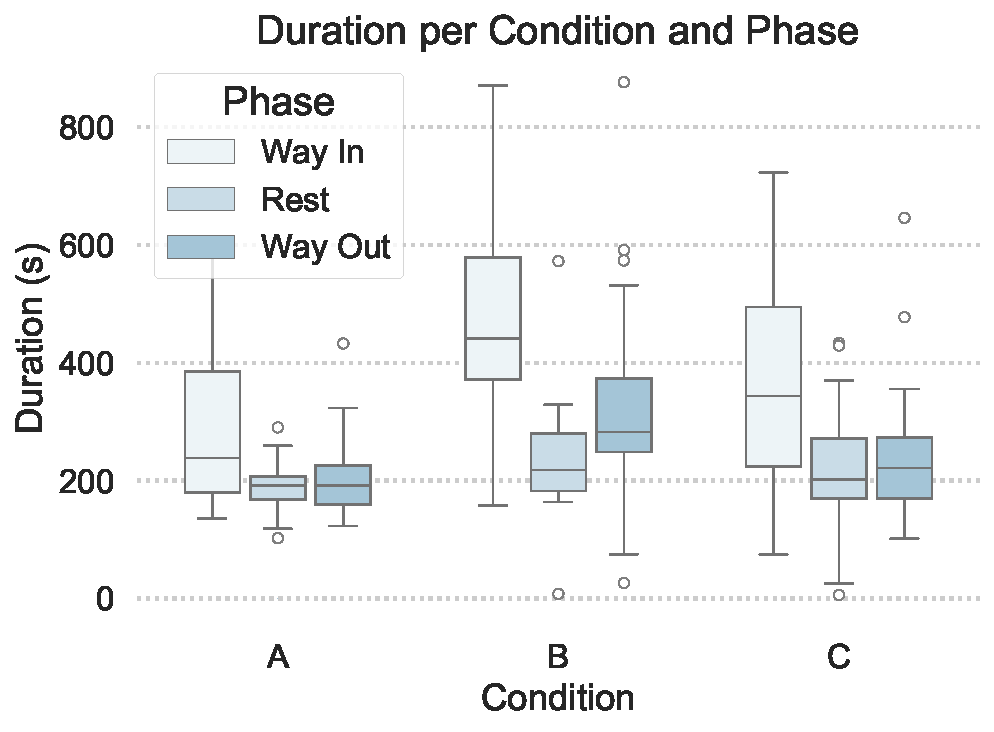
\includegraphics[width=\textwidth]{include/images/duration_per_phase.pdf}
		\caption{Duration per phase}
		\label{fig:duration-phase}
	\end{subfigure}
	\captionsetup{subrefformat=parens}
	\caption[Results: duration]{Time participants took for completing the conditions and their inherent phases}
	\label{fig:duration}
\end{figure} 

\subsection{Duration}

We conducted repeated measures \glspl{ANOVA} to examine the effect of the condition on time that participants took to complete the tasks. Regarding the duration per conditions (Figure \ref{fig:duration-condition}), there was a significant effect of condition on duration (N = 23): \fdf{2}{44}{9.092}, \psig{<}{0.01}. The effect has an observed power of 0.966 with \peta{0.292}; a correction for sphericity was not necessary (\chisq{0.872}, \psig{=}{0.188}). Pairwise Bonferroni Tests showed significant differences between \ref{cd:A} and \ref{cd:B} (\psig{<}{0.01}), \ref{cd:A} and \ref{cd:C} (\psig{<}{0.05}), but not between \ref{cd:B} and \ref{cd:C} (\psig{=}{0.575}). There was no coherent effect of the phase across all phases (Figure \ref{fig:duration-phase}). On average, it took the subjects \SI{4}{\minute} (SD = 1), \SI{6}{\minute} (SD = 2), and \SI{5}{\minute} (SD = 2) to climb the traverses in \ref{cd:A}, \ref{cd:B}, and \ref{cd:C}, respectively. \pdfmargincomment[avatar=peter,style=korrektur-done]{überarbeitet}

\subsection{Physical Exertion}

In the first place, we recorded the vital signs \gls{HR}, \gls{RR} because they are indicators for physical exertion, a criterion we used to group conditions. \gls{HR} was measured using an \gls{ECG} in combination with a chest strap, to obtain reference signal less prone to motion artifacts. The results can be seen in Figure \vref{fig:physical-exertion}.

\begin{figure}[htb]
	\centering
	\begin{subfigure}[t]{0.49\columnwidth}
		\centering
		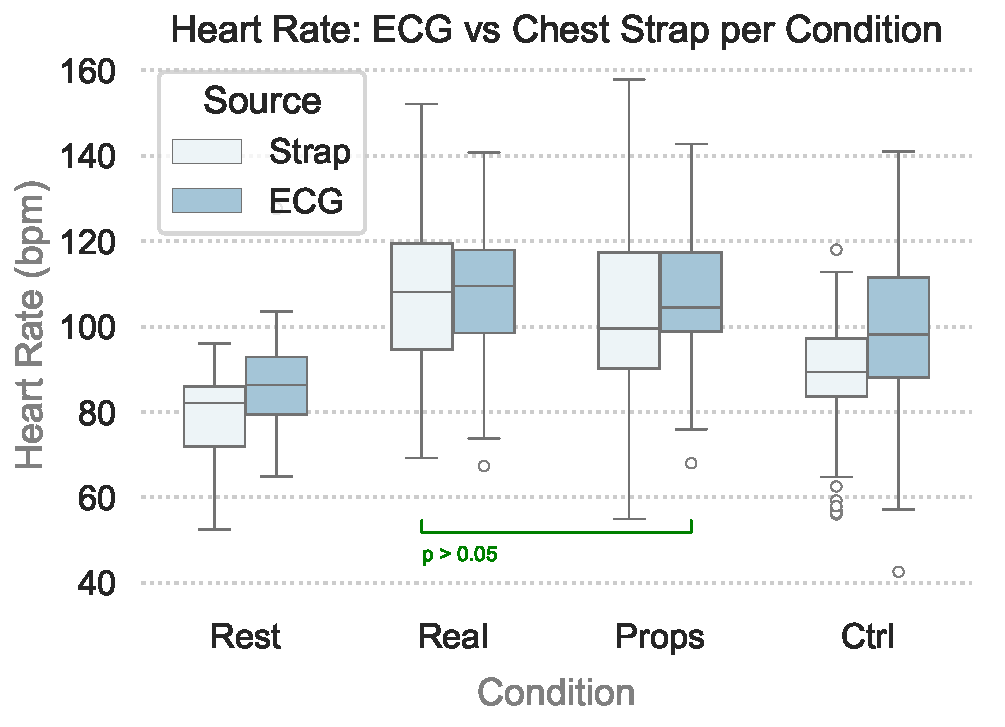
\includegraphics[width=\textwidth]{include/images/hr_per_condition_by_source.pdf}
		\label{fig:physical-exertion-hr}
	\end{subfigure}
	\hspace*{\fill}
	\begin{subfigure}[t]{0.49\columnwidth}
		\centering
		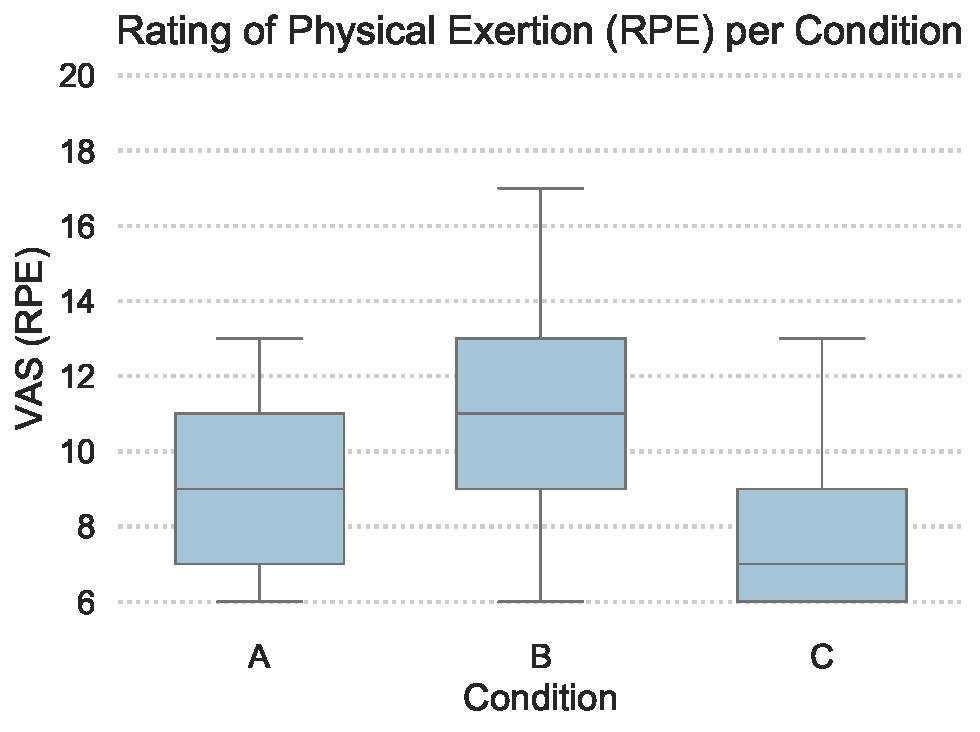
\includegraphics[width=\textwidth]{include/images/rpe_per_condition.pdf}
		\label{fig:physical-exertion-rpe}
	\end{subfigure}
	\label{fig:physical-exertion}
\end{figure}

We conducted a repeated measures \gls{ANOVA} to examine the effect of the condition on \gls{HR} for both sources. For \textbf{\gls{ECG}}-based \gls{HR} (N = 23), Mauchly's Test of Sphericity indicated that the assumption of sphericity had not been violated, \chisq{5.866}, \psig{=}{0.320}. There was a significant effect of condition on \gls{HR}: \fdf{3}{63}{22.502}, \psig{<}{0.01}. The effect has an observed power of 1.0 with \peta{0.517}. For the recordings from the \textbf{chest strap} (N = 22), Mauchly's Test of Sphericity indicated a violation of sphericity, \chisq{12.653}, \psig{<}{0.05}, and therefore, a Greenhouse-Geisser correction was used. There was a significant effect of condition on \gls{HR}: \fdf{2.192}{46.035}{92.877}, \psig{<}{0.01}. The effect has an observed power of 1.0 with \peta{0.816}. A pairwise Bonferroni Test of the conditions revealed that the mean \gls{HR} is different in condition except for \ref{cd:A} and \ref{cd:B} (\psig{>}{0.05}), for both sources.

Since the \gls{RPE} yields discrete, ordinal results, we used a Friedman Test to examine the effect of condition on self-reported physical exertion. There was a significant effect of condition on \gls{RPE}, $\chi^2$ = 23.234, \psig{<}{0.01}. A pairwise Wilcoxon Signed Ranks Test revealed a significant difference for \ref{cd:A} and \ref{cd:B} (Z = -2.517, \psig{=}{0.012}), \ref{cd:A} and \ref{cd:C} (Z = -2.340, \psig{=}{0.019}), and \ref{cd:B} and \ref{cd:C} (Z = -3.817, \psig{<}{0.01}).

\subsection{Stress and Anxiety}

For anxiety we used the \gls{ECG} signal and derived the \gls{mRRI} from it as a measure of \gls{HRV}. Further, we measured \gls{EDA} and derived the \gls{SCR}-level from it. To examine the effect of the condition on each measure, we conducted a repeated measures \gls{ANOVA}. For \textbf{\gls{mRRI}} (N = 21), Mauchly's Test of Sphericity indicated a violation of sphericity, \chisq{16.401}, \psig{<}{0.05}, and therefore, a Greenhouse-Geisser correction was used. There was a significant effect of condition on \gls{mRRI}: \fdf{2.036}{40.719}{4.331}, \psig{<}{0.05}. The effect has an observed power of 0.725 with \peta{0.178}. A pairwise Bonferroni Test revealed only a significant difference between \ref{cd:0} and \ref{cd:B} (\psig{<}{0.01}).

To examine \gls{SC}, we looked at two the \glspl{NSR}: response-count and conductivity level \autocite{SkinConductivityExplained}. The first was calculated from the rolling average of detected peaks within a \SI{20}{\second} time-frame. Neither the response count nor the level did show any patterns. So unlike the \gls{HRV}, we could not find any significant differences between the conditions for the \textbf{\gls{EDA} signals}.

\begin{figure}[htb]
	\centering
	\begin{subfigure}[t]{0.49\columnwidth}
		\centering
		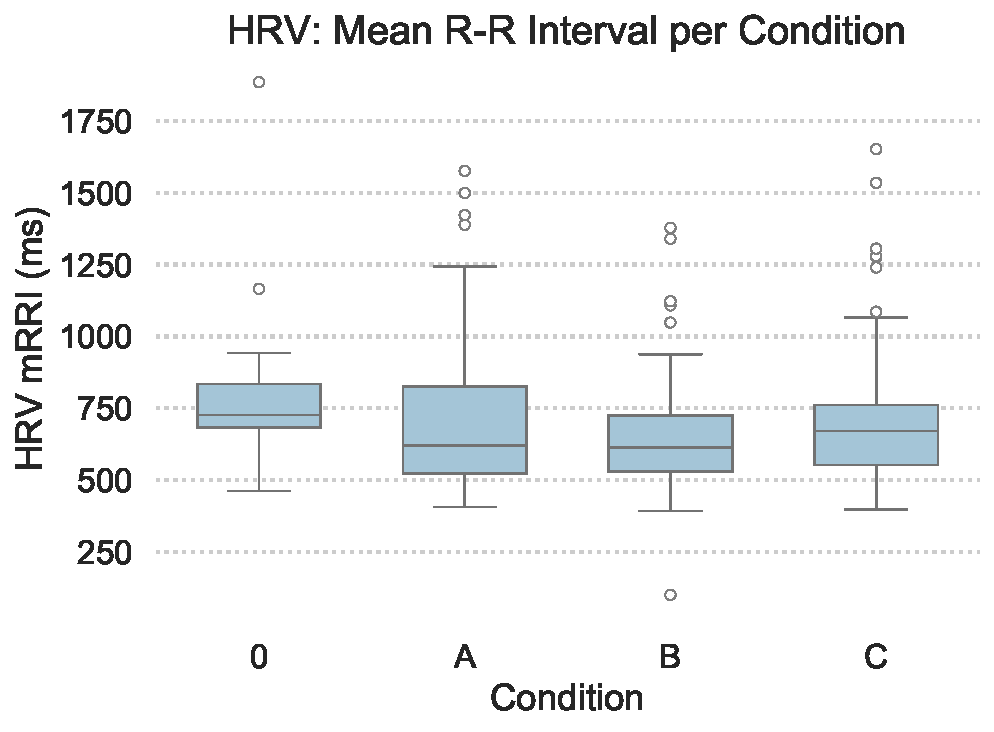
\includegraphics[width=\textwidth]{include/images/hrv_per_condition.pdf}
		\label{fig:stress-hrv}
	\end{subfigure}
	\hspace*{\fill}
	\begin{subfigure}[t]{0.49\columnwidth}
		\centering
		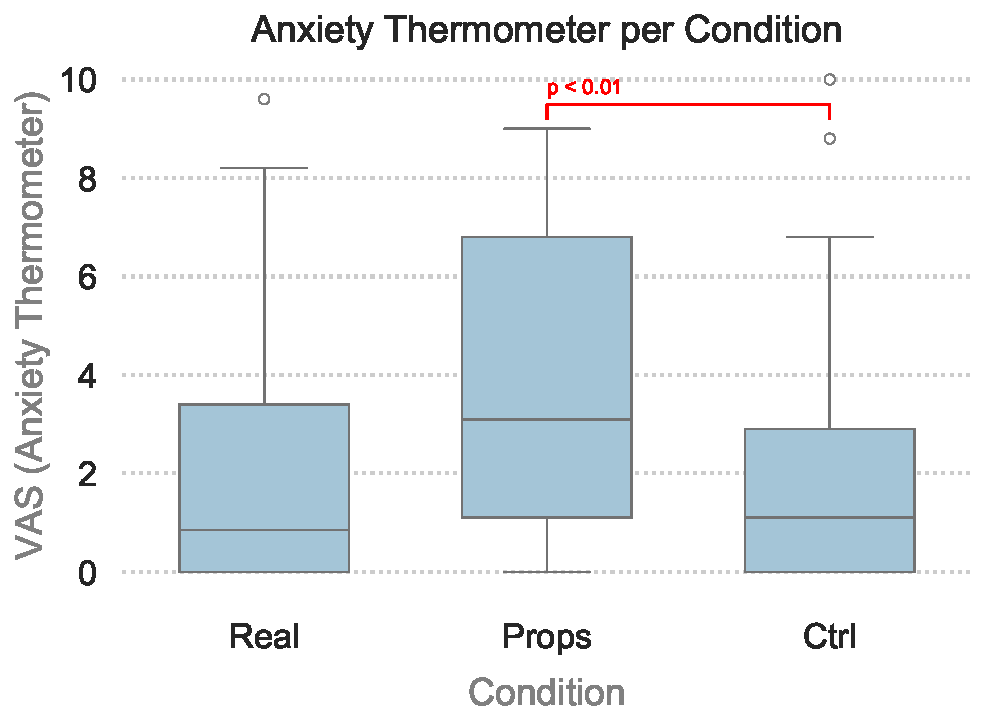
\includegraphics[width=\textwidth]{include/images/at_per_condition.pdf}
		\label{fig:anxiety-at}
	\end{subfigure}
	\label{fig:stress-anxiety}
\end{figure}

In contrast to \gls{RPE}, the \gls{VAS} \glsfirst{AT} uses a continuous scale. We could conduct a repeated measures \gls{ANOVA} without correction (\chisq{0.692}, \psig{=}{0.708}). There was a significant effect of condition on self-reported anxiety, \fdf{2}{44}{5.364}, \psig{<}{0.05}. The effect has an observed power of 0.815 with \peta{0.195}. A pairwise Bonferroni Test of the conditions revealed that the mean \gls{AT} response for \ref{cd:B} is significantly higher than for \ref{cd:C} (\psig{<}{0.01}).

\subsection{Presence}

Finally, after conditions \ref{cd:B} and \ref{cd:C}, the participants rated their sense of presence through an \gls{IPQ} questionnaire (N = 27); the results can be seen in Figure \ref{fig:presence}. To examine the effect of the condition on presence scores, we conducted paired t-tests. There only was a significant effect of the condition on realness (REAL) scale with t(26) = 2.621, \psig{=}{0.014}. The effect has an observed power of 0.714 with \peta{0.209}. As suggested by \textcite{Meehan2001} we also examined the rolling average of the \gls{HR}---using a window of two respiration cycles---but that did not show any significant differences between the conditions.

\begin{figure}[htb]
   \begin{center}
   	   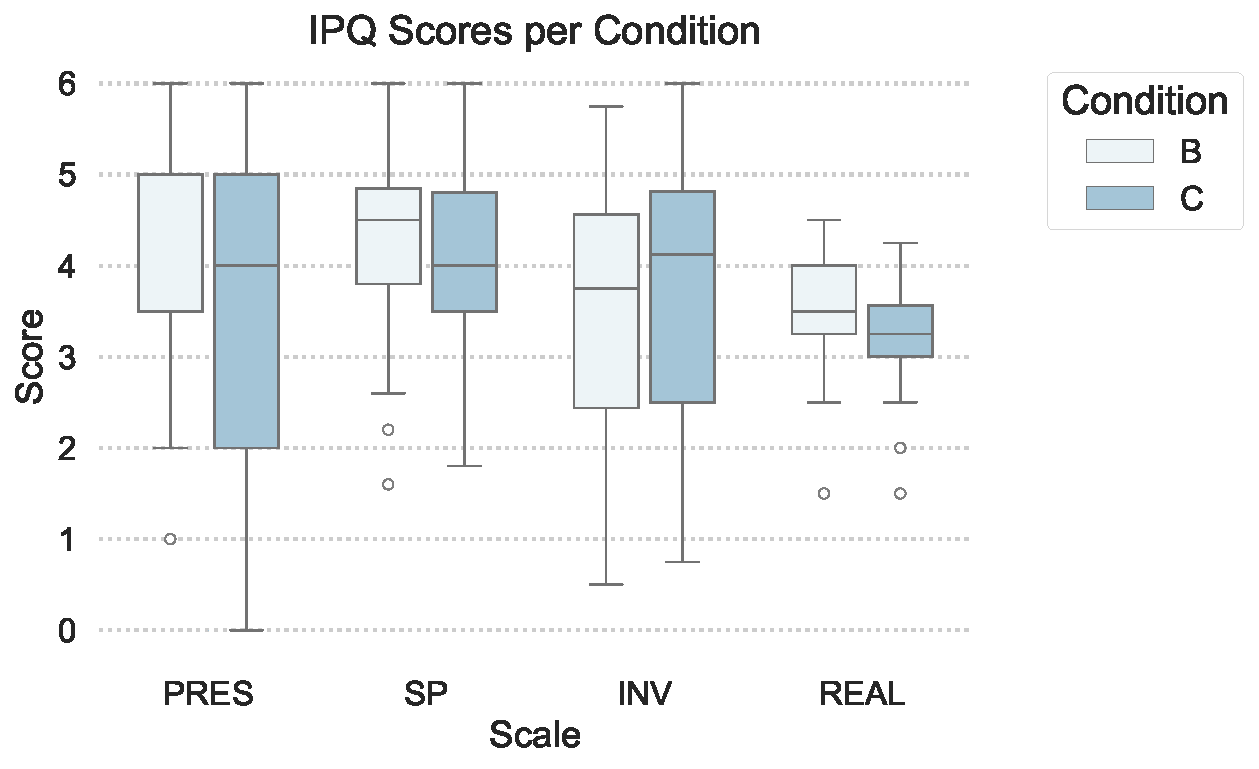
\includegraphics[width=0.6\textwidth]{include/images/ipq_per_condition}
   	\captionsetup{subrefformat=parens}
   	\caption{\gls{IPQ} Werte für die Bedingungen B und C auf den Skalen \textit{general presence} (PRES), \textit{spatial awareness} (SP), \textit{involvement} (INV), and \textcolor{secondary}{\textit{realness} (REAL)}}
   	\label{fig:presence}
   \end{center}
\end{figure}

The authors of the \gls{IPQ} offer a database with results from multiple studies \autocite{IPQDatabase2016}. This dataset includes 37 records for experiments with 3D graphics displayed via \gls{HMD}. Considering these, we found higher scores than those in the database on all scales. However, the differences were significant only for spatial awareness (SP) and realness (REAL)  in condition \ref{cd:B} (Δ\textsubscript{SP} = 1.007, p < 0.01; Δ\textsubscript{REAL} = 1.596, p < 0.01) and \ref{cd:C} (Δ\textsubscript{SP} = 1, p < 0.01; Δ\textsubscript{REAL} = 1.328, p < 0.01).

\subsection{Qualitative Feedback}

After each run, we asked the subjects to comment on what they had just experienced and took notes of them. Here is a list of statements ordered by frequency:
\begin{itemize*}[itemjoin={{, }},itemjoin*={{, and }},noitemsep,nolistsep]
	\item[] “It felt like being up there [on the high platform.]”: 6 times
	\item[] “Climbing [in VR] felt more realistic [than using the controllers.]”: 6 times
	\item[] “The scene was very real.”: 5 times
	\item[] “My feet were off a bit.”: 4 times
	\item[] “I was not sure if I can trust the [\gls{VR}] technology.”: 3 times
	\item[] “I was more anxious, because I was not fixed to a rope [in \gls{VR}.]”: twice
	\item[] “Tracking was lost.”: twice
	\item[] “I had a gut feeling [when standing on the high platform].”: once
    \item[] “I could not see my hands, now and again.”: once
    \item[] “I didn't feel like being up there [on the high platform] at all.”: once
\end{itemize*}

 % Please add the following required packages to your document preamble:
% \usepackage{booktabs}
\begin{landscape}
\begin{table}[!b]
\centering
\caption[Results: measurements]{Overview of the measured values for the conditions \ref{cd:0} to \ref{cd:C}; N varies due to incomplete or missing recordings and answers}
\label{tab:measurement-results}
\tablestyle{%
	\begin{tabu}  to \textheight {%
			@{}
			X[1]
			S[table-format=2]
			S[table-format=3.2]
			S[table-format=3.2]
			S[table-format=3.2]
			S[table-format=3.2]
			S[table-format=3.2]
			S[table-format=3.2]
			S[table-format=3.2]
			S[table-format=3.2]
			@{}}
		\toprule
      &    & \multicolumn{2}{l}{\textbf{\ref{cd:0}}} & \multicolumn{2}{l}{\textbf{\ref{cd:A}}} & \multicolumn{2}{l}{\textbf{\ref{cd:B}}} & \multicolumn{2}{l}{\textbf{\ref{cd:C}}} \\
		\textbf{Measurement}    & \multicolumn{1}{l}{\textbf{N}}  & \multicolumn{1}{l}{\textbf{Mean}}      & \multicolumn{1}{l}{\textbf{SD}}        & \multicolumn{1}{l}{\textbf{Mean}}      & \multicolumn{1}{l}{\textbf{SD}}        & \multicolumn{1}{l}{\textbf{Mean}}      & \multicolumn{1}{l}{\textbf{SD}}        & \multicolumn{1}{l}{\textbf{Mean}}      & \multicolumn{1}{l}{\thead{SD}} \\\midrule
		duration (s) & 23 & 418.72 & 281.24 & 231.08 & 62.84 & 358.75 & 133.47 & 310.84 & 106.76\\
		\gls{HR} from \gls{ECG} (bpm)   & 23 & 86.11     & 13.27     & 108.71    & 11.50     & 108.07    & 9.71      & 98.42     & 15.33     \\
		\gls{HR} from Chest Strap (bpm) & 22 & 79.75     & 11.77     & 107.82    & 16.91     & 102.96    & 15.62     & 88.18     & 12.98     \\
		\gls{RR} (Hz)        & 23 & 0.26      & 0.03      & 0.21      & 0.02      & 0.22      & 0.02      & 0.22      & 0.02      \\
		\gls{HRV} \gls{mRRI} (ms)  & 21 & 769.40    & 132.89    & 700.43    & 195.72    & 605.63    & 78.50     & 708.70    & 174.20    \\
		\gls{EDA} as \gls{SCR} peaks (count) & 22 & 8.00   & 3.30   & 5.80   & 2.25   & 6.26   & 2.34   & 6.51   & 2.02  \\
		\textbf{\glspl{VAS}}            &    &           &           &           &           &           &           &           &           \\ \tabucline[sline]{1-10}
		\gls{RPE} (6 to 20)            & 28 &           &           & 9.46      & 2.32      & 11.04     & 3.07      & 7.89      & 2.41      \\
		\gls{AT} (0 to 10)            & 23 &           &           & 2.43      & 2.87      & 3.94      & 2.85      & 1.95      & 2.26      \\
		\textbf{\gls{IPQ}}            &    &           &           &           &           &           &           &           &           \\ \tabucline[sline]{1-10}
		general presence (PRES)           & 27 &           &           &           &           & 4.15      & 1.75      & 3.44      & 1.91      \\
		spatial awareness (SP)             & 27 &           &           &           &           & 4.24      & 1.13      & 3.96      & 1.07      \\
		involvement (INV)            & 27 &           &           &           &           & 3.44      & 1.54      & 3.76      & 1.40      \\
		realness (REAL)           & 27 &           &           &           &           & 3.58      & 0.54      & 3.31      & 0.52      \\ \bottomrule
	\end{tabu}}
\end{table}
\end{landscape}